\section{ARMA Processes}


A time series $\{Y_t\}_{t\in\mathbb{Z}}$ is a linear process if, for all $t$, $Y_t = \sum_{j=-\infty}^{\infty}\psi_jY_{t-j}$ and $\sum_{j=-\infty}^\infty |\psi_{t-j}|$ converges. We can express $Y_t$ with $\sum_{j=-\infty}^{\infty}\psi_jB^jY_{t}$, introducing the backwards operator $B$, which behaves as follows: $(B^a)Y_t = Y_{t-a}$. A stationary time series $\{Y_t\}$ is an  auto-regressive moving average process of order $p,q$ (denoted ARMA$(p,q)$)  if it is expressible as:

\begin{equation}
    \label{eq:ARMA}
    \phi(B)Y_t = \theta(B)Z_t, \qquad Z_t \sim WN(0,\sigma^2),
\end{equation}
in which $\phi(B)$ and $\theta(B)$ are polynomials in $B$ of orders $p$ and $q$, respectively. Importantly, the two polynomials must share no common roots and have no roots of magnitude 1. The process is \textit{causal} if all roots of $\phi(B)$ are of magnitude strictly less than 1, as this will result in $\psi_j = 0$ for all $j<0$, meaning $Y_t$ is only a function of ``past'' values. The time series is \textit{reversible} if all roots of $\theta(B)$ are of magnitude strictly less than 1. We will be restricting the scope of this dissertation to causal, reversible ARMA processes for which $p,q \leq1$. It will therefore always be the case that $|\phi|,|\theta|<1$.

If $\{Y_t\}$ is an AR(1) process, it is defined by the equation $Y_t-\phi Y_{t-1} = Z_t$ with $Z_t \overset{\text{i.i.d.}}{\sim}\text{WN}(0,\sigma^2)$ and has the following auto-covariance function:

\begin{equation}
    \label{eq:acvf_ar}
    \gamma_Y(h) = \frac{\sigma^2\phi^{|h|}}{1-\phi^2}, \qquad h \in \mathbb{Z}
\end{equation}



\begin{figure}[htbp]

  % Top image (row 1)
  \begin{subfigure}{.45\textwidth}
    \centering
    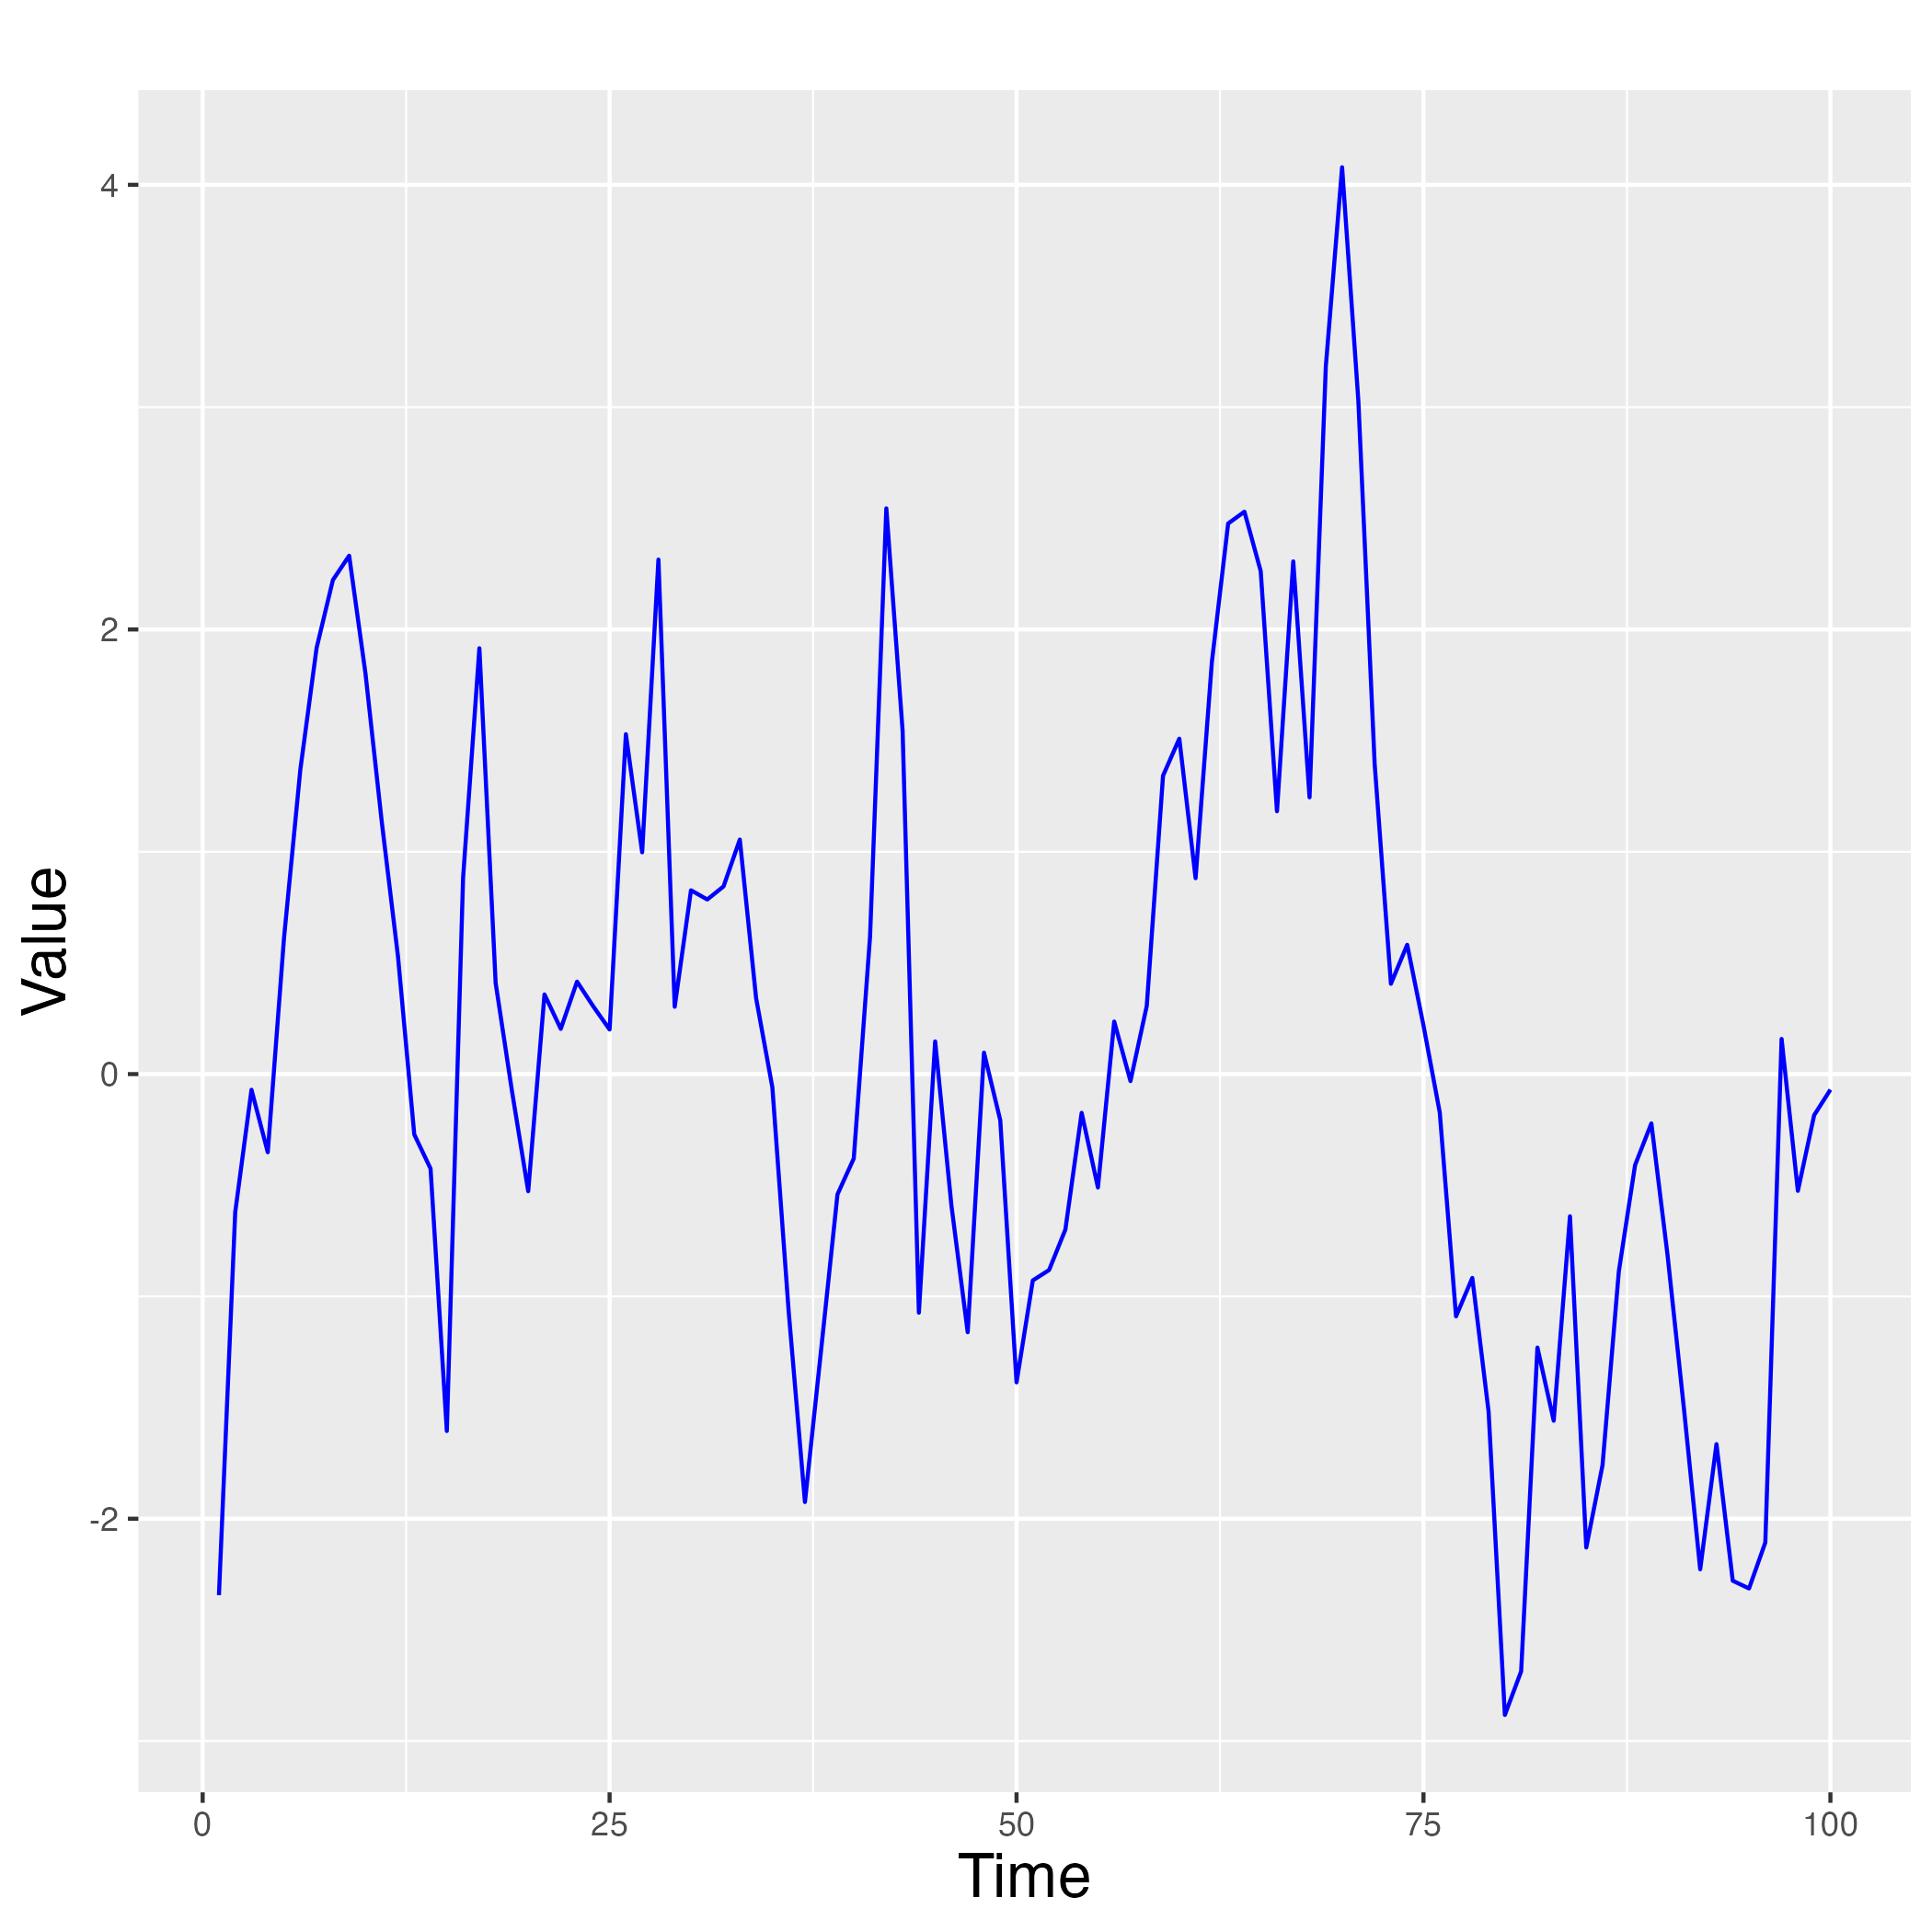
\includegraphics[width=\textwidth]{images/output/ar_ex.png}
    \caption{Realization}
  \end{subfigure}
  \hfill
  % Bottom image (row 2)
    \begin{subfigure}{0.45\textwidth}
        \centering
        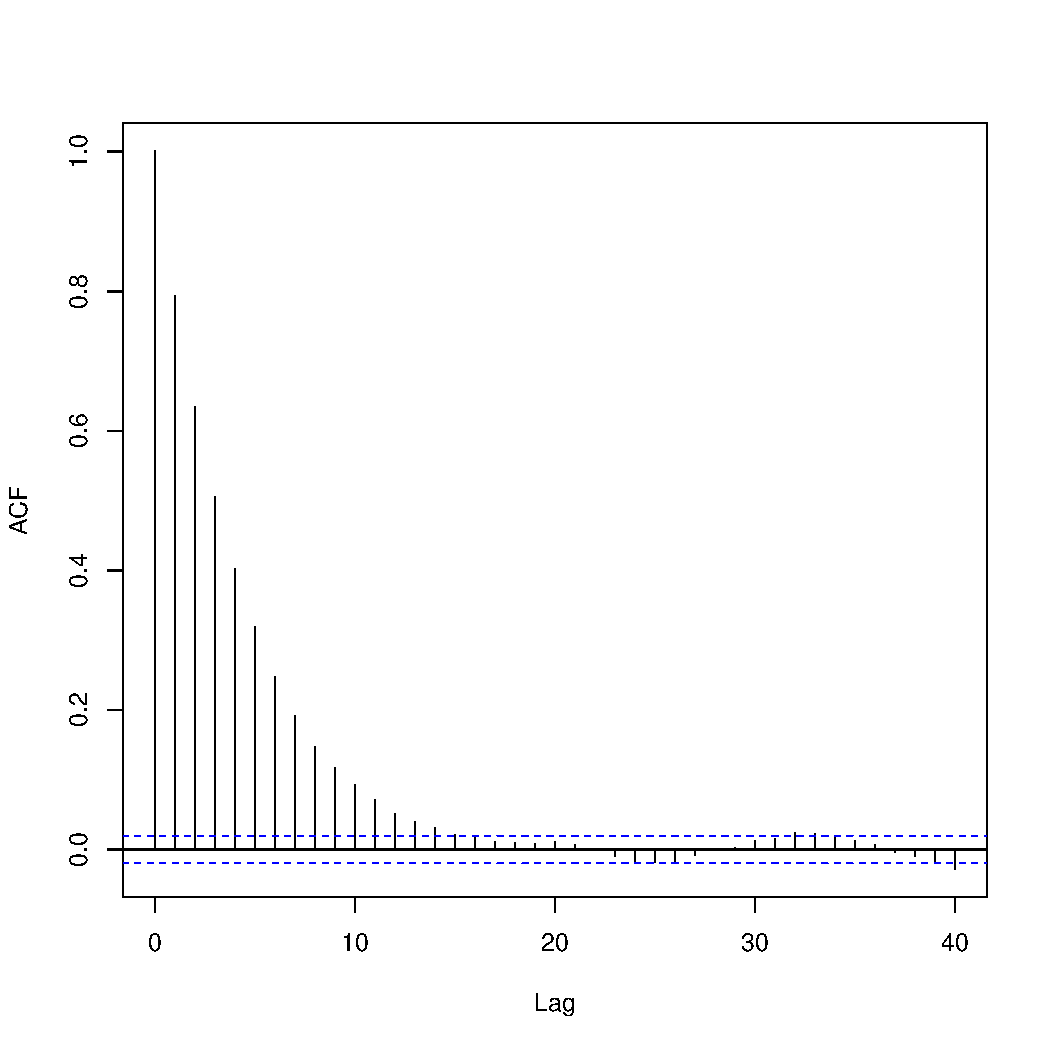
\includegraphics[width=\linewidth, page=1]{images/output/sample_acf.pdf}
        \caption{SACF}
    \end{subfigure}
  \caption{Sample AR(1) Process with $(\phi,\sigma^2) = (0.8, 1)$}
  \label{fig:sample_ar_pos}
\end{figure}

In Figure \ref{fig:sample_ar_pos}, we see a sample AR(1) process with a strong positive coefficient. By contrast, an AR(1) with a strong negative coefficient will oscillate rapidly, as shown in Figure \ref{fig:sample_ar_neg}.

\begin{figure}[]
    \centering
      \begin{subfigure}{.45\textwidth}
    \centering
    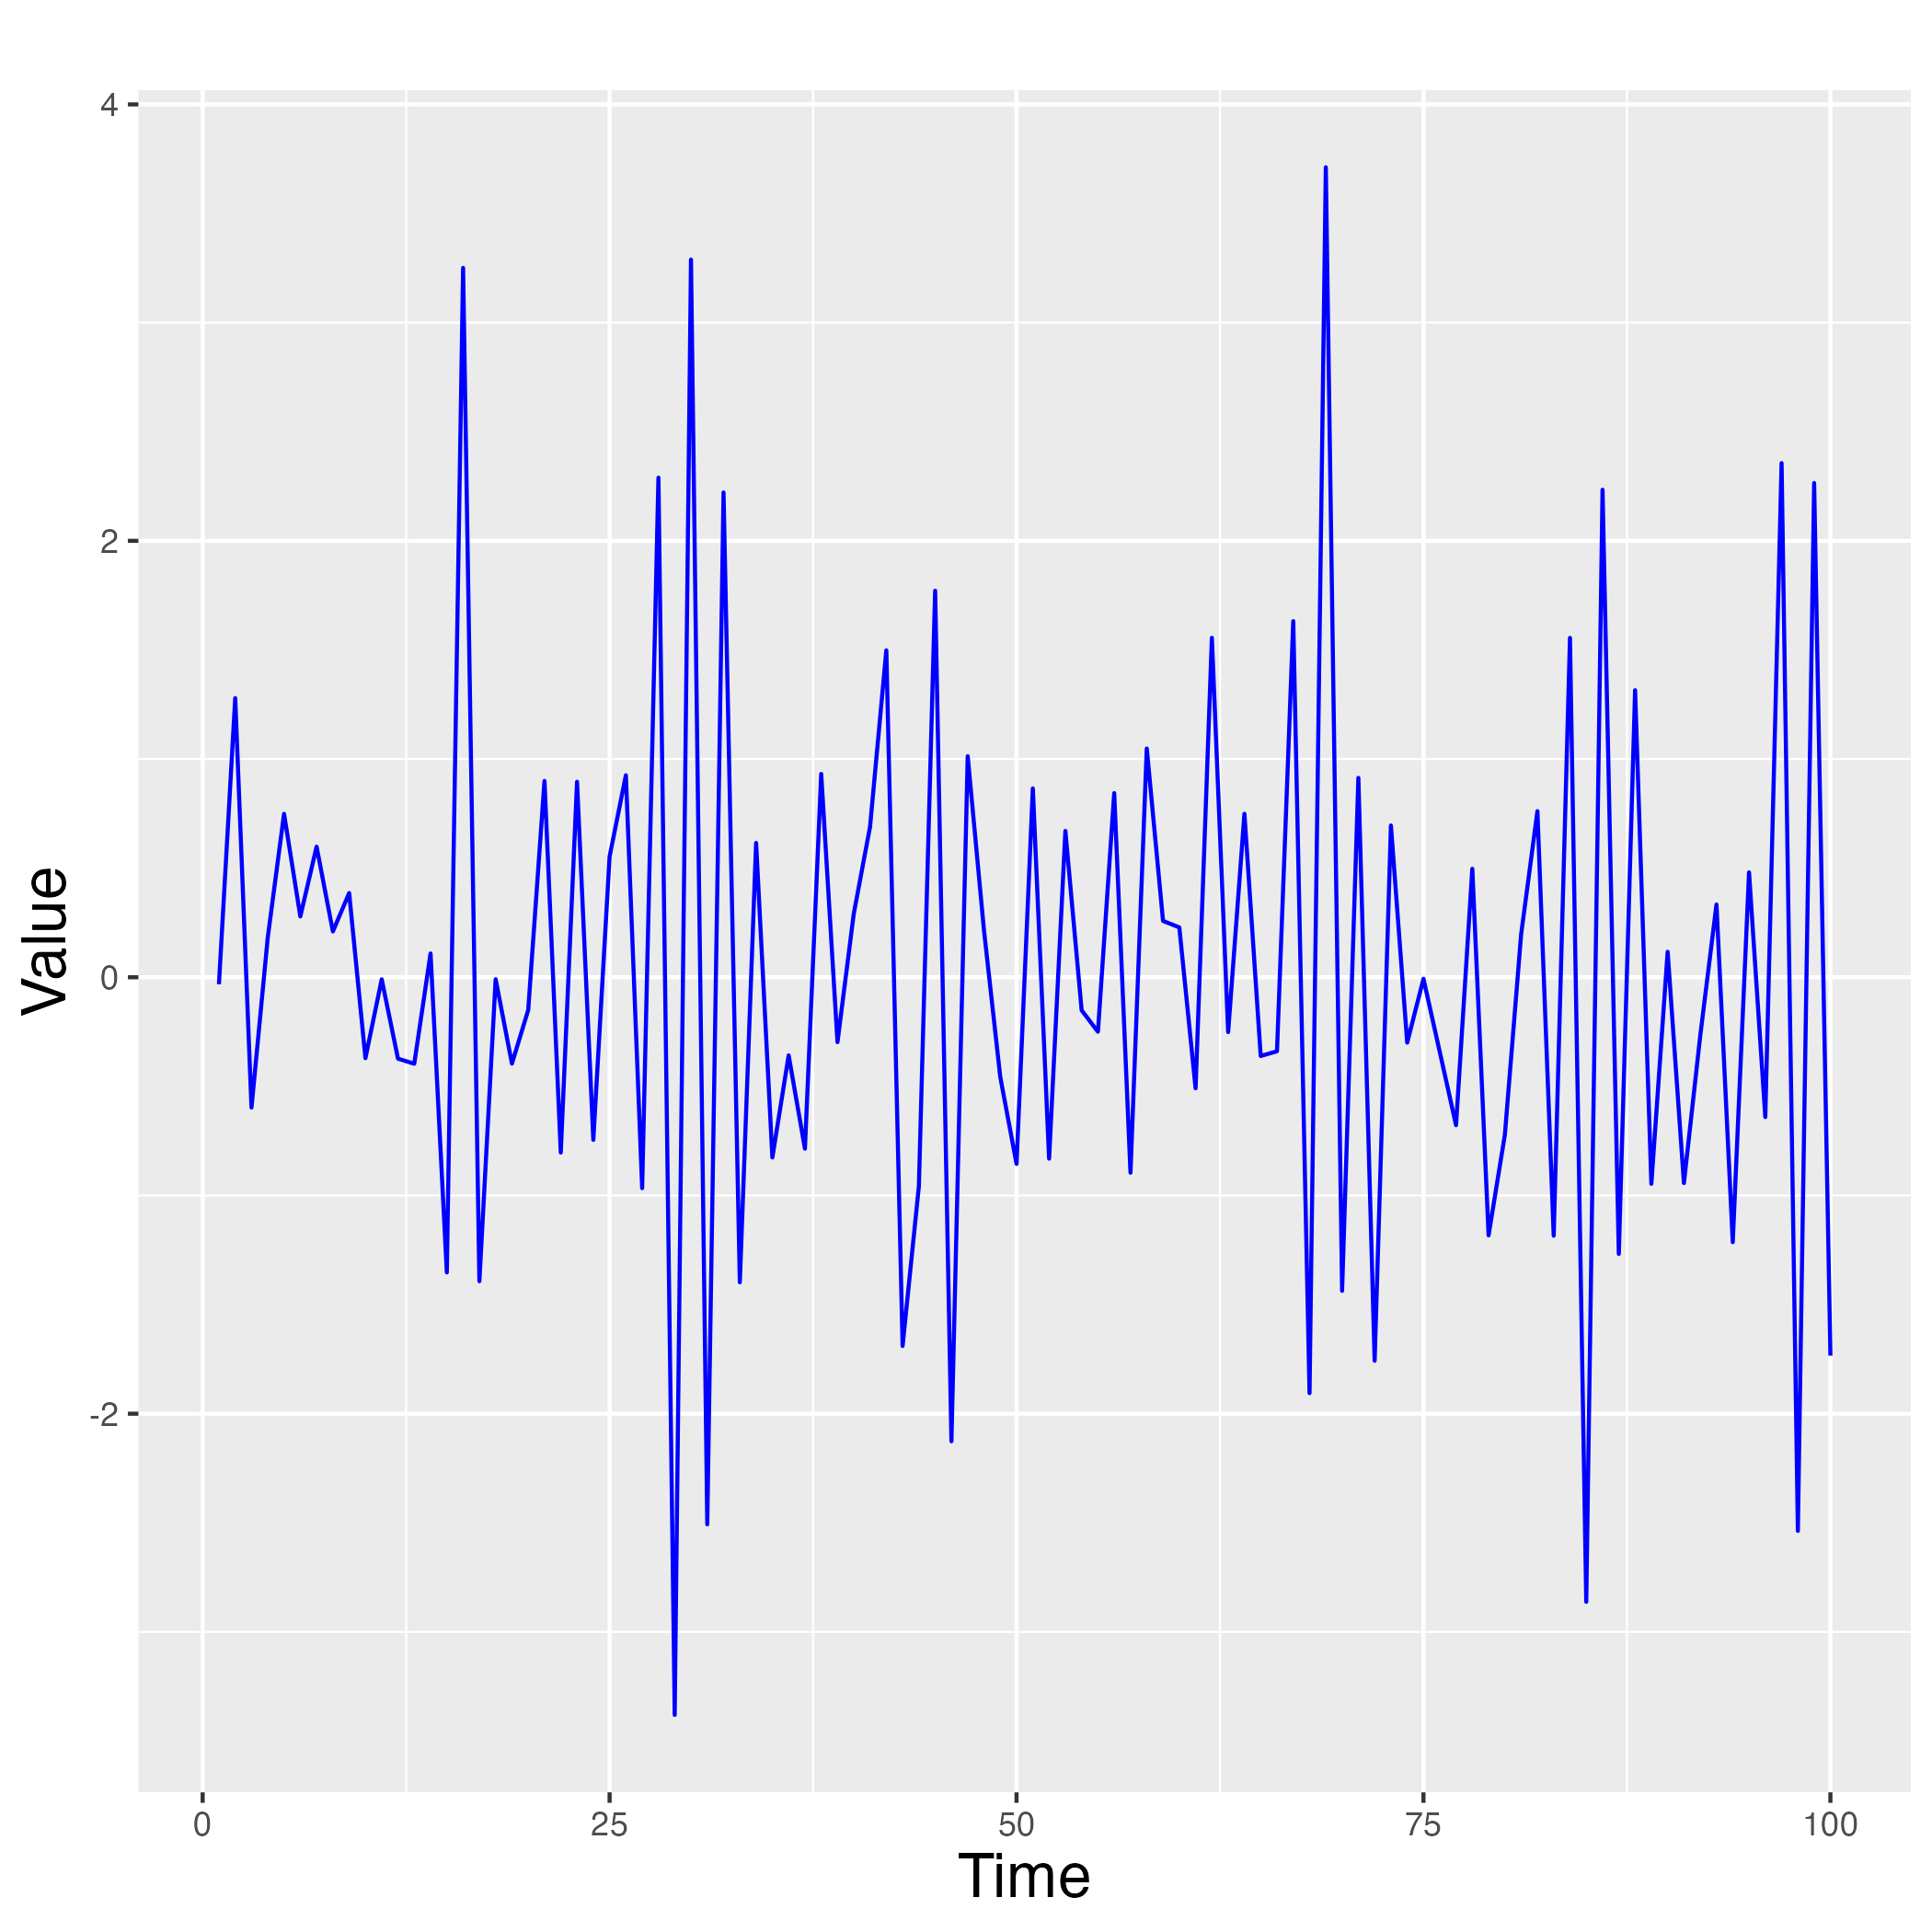
\includegraphics[width=\textwidth]{images/output/ar_neg_ex.png}
    \caption{Realization}
    \label{fig:img2}
  \end{subfigure}
f    \hfill
    \begin{subfigure}{0.45\textwidth}
        \centering
        \includegraphics[width=\linewidth, page=2]{images/output/sample_acf.pdf}
        \caption{SACF}
    \end{subfigure}
    \caption{Sample AR(1) Process with $(\phi, \sigma^2) = (-0.8,1)$}
    \label{fig:sample_ar_neg}
\end{figure}


An MA(1) process, which can be expressed as an equation of the form $Y_t = Z_t + \theta Z_t, \hspace{.1in}\{Z_t\}\sim \text{WN}(0,\sigma^2)$ has the following ACVF:

\begin{equation}
    \label{eq:acvf_ma}
    \gamma_Y(h) = \begin{cases}
        (1 + \theta^2)\sigma^2 & h = 0 \\
        \theta\sigma^2 & |h| = 1 \\
        0 & \text{else}
    \end{cases}
\end{equation}

Figures \ref{fig:sample_ma_pos} and \ref{fig:sample_ma_neg} illustrate MA(1) processes with $\sigma^2 = 1$ and $\theta = 0.8$ and $\theta = -0.8$, respectively.


\begin{figure}[htbp]

  % Top image (row 1)
  \begin{subfigure}{.45\textwidth}
    \centering
    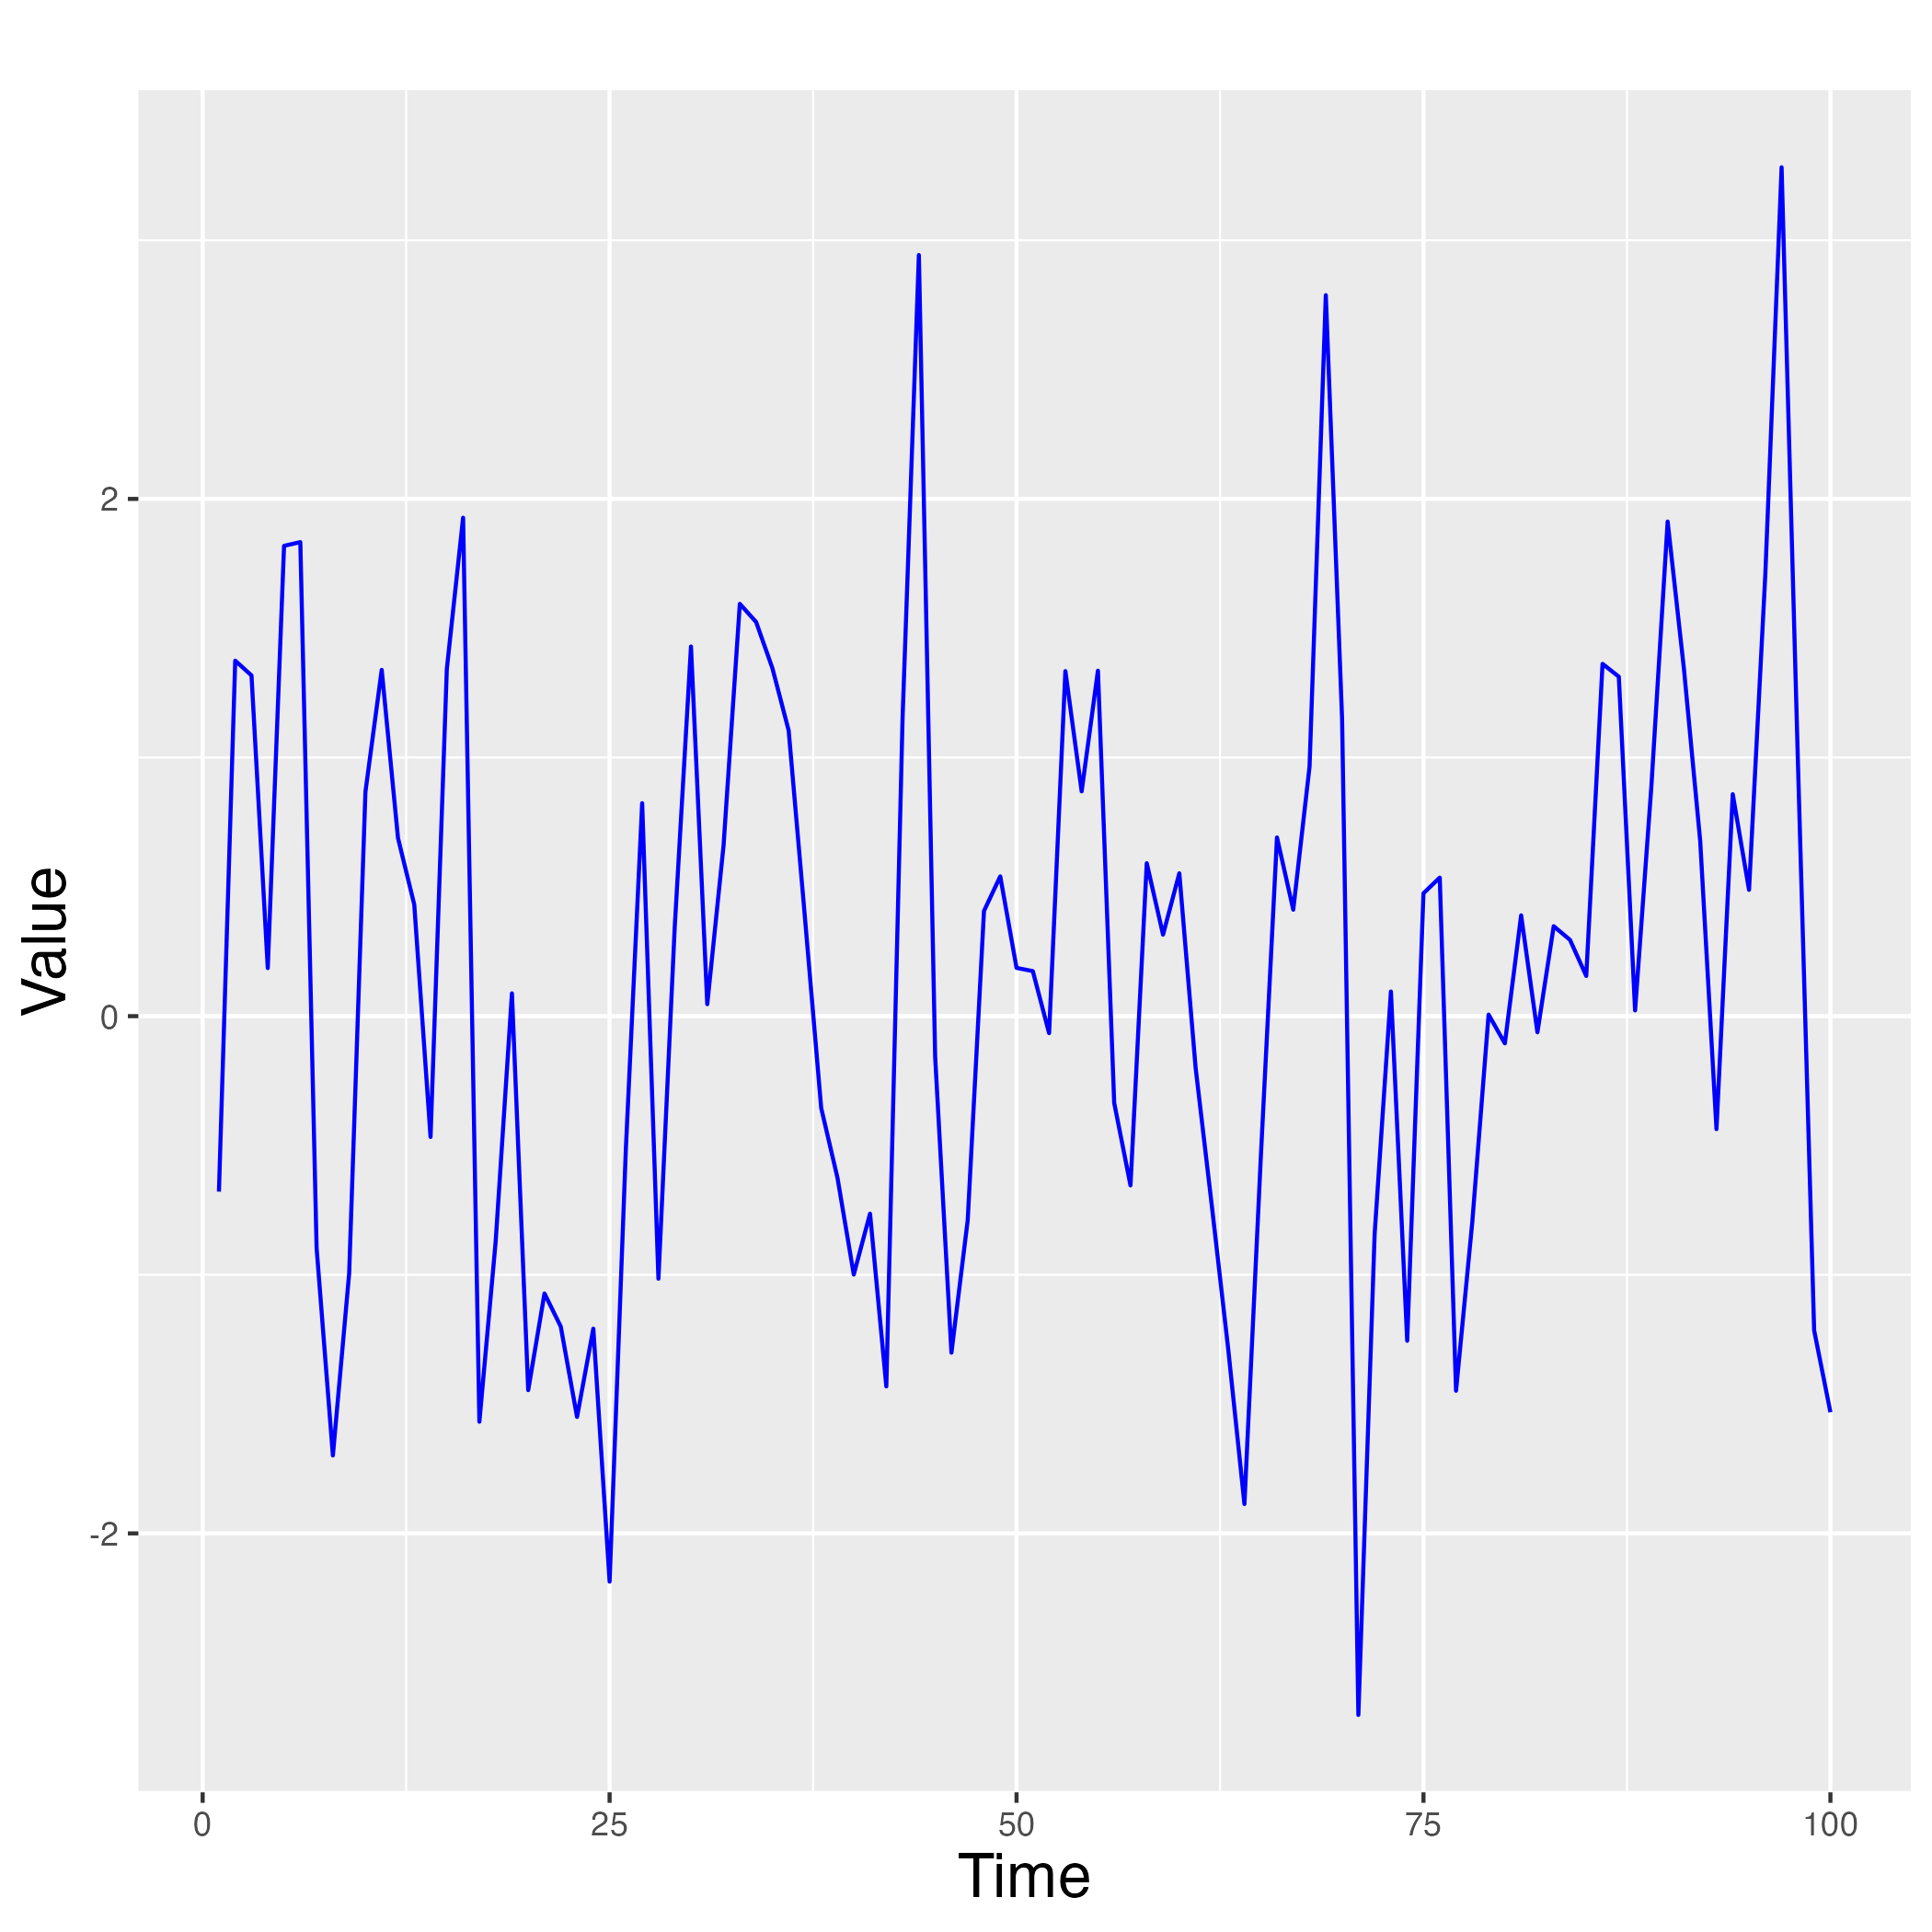
\includegraphics[width=\textwidth, trim={0 0 0 .5cm}, clip]{images/output/ma_ex.png}
    \caption{Realization}
    \label{fig:img1}
  \end{subfigure}
  \hfill
    \begin{subfigure}{0.45\textwidth}
        \centering
        \includegraphics[width=\linewidth,page=3]{images/output/sample_acf.pdf}
        \caption{SACF}
    \end{subfigure}
  % Bottom image (row 2
  \caption{Sample MA(1) Process with $(\theta,\sigma^2) = (0.8,1)$}
  \label{fig:sample_ma_pos}
\end{figure}



\begin{figure}
    \centering
    \begin{subfigure}{.45\textwidth}
    \centering
    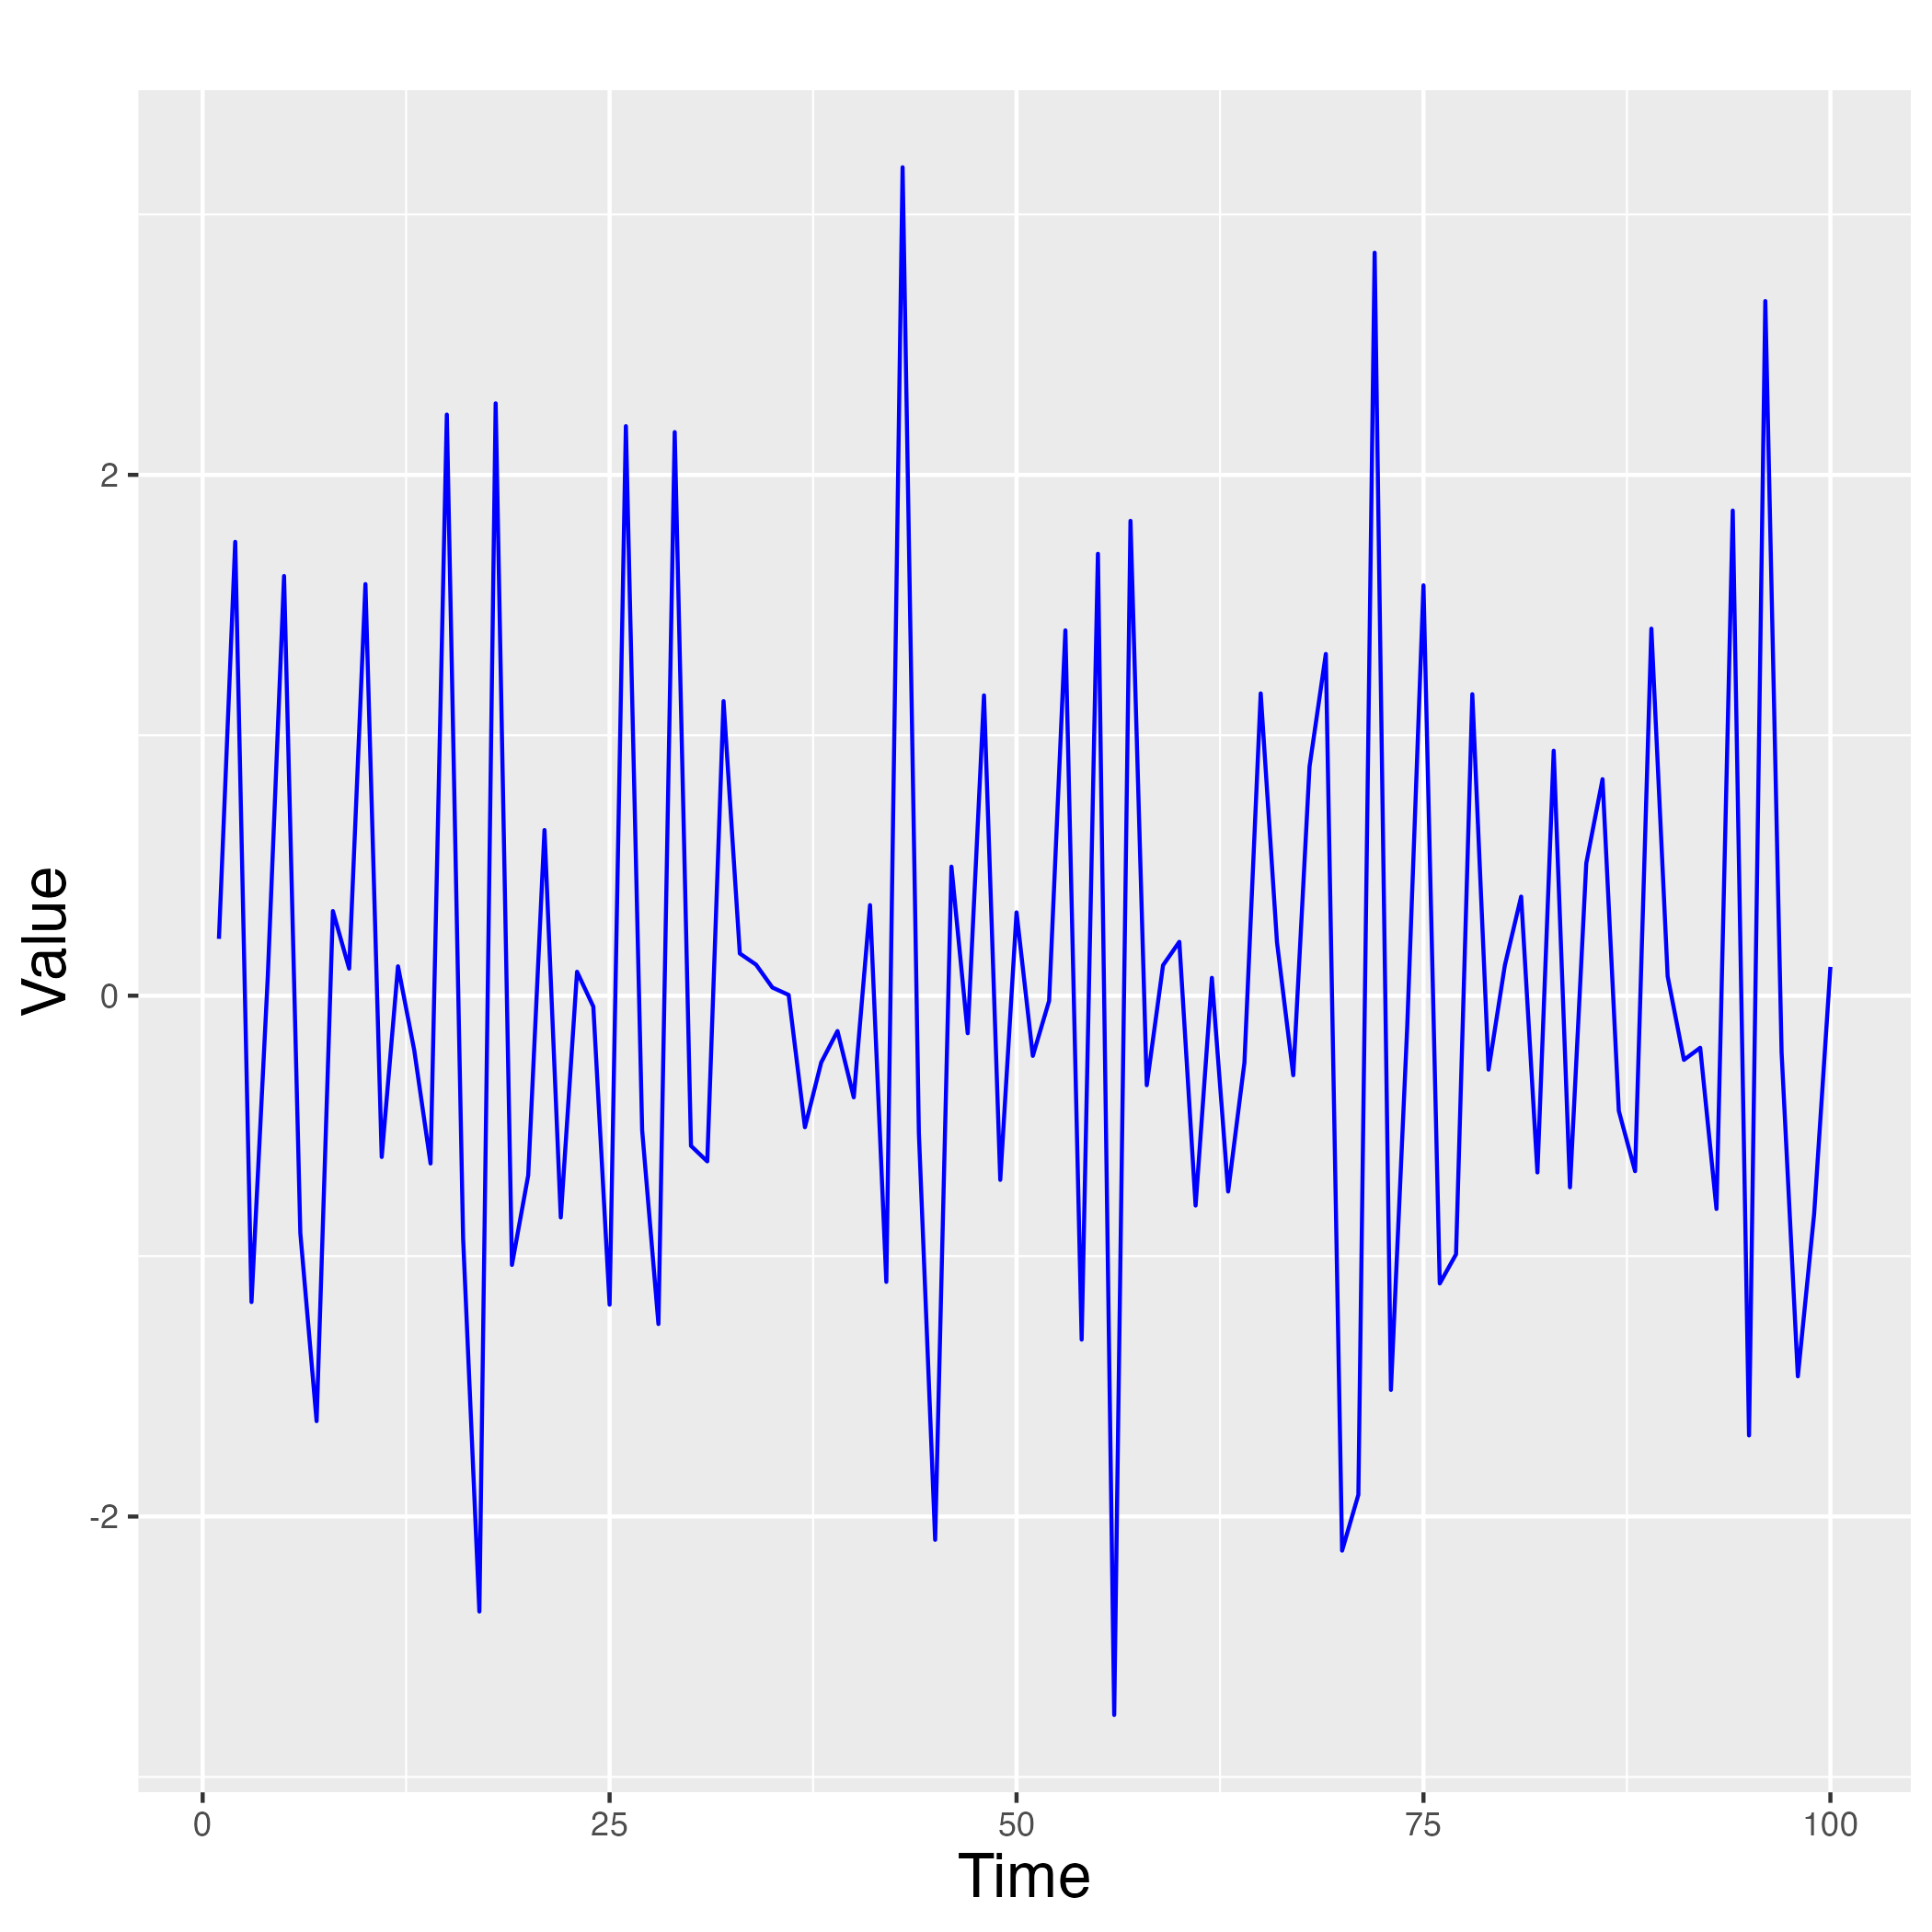
\includegraphics[width=\textwidth]{images/output/ma_neg_ex.png}
    \caption{Realization}
    \label{fig:img2}
  \end{subfigure}
    \hfill
    \begin{subfigure}{0.45\textwidth}
        \centering
        \includegraphics[width=\linewidth, page=4]{images/output/sample_acf.pdf}
        \caption{SACF}
    \end{subfigure}
    \caption{Sample MA(1) Process with $(\theta, \sigma^2) = (-0.8,  1)$}
    \label{fig:sample_ma_neg}
\end{figure}




An ARMA(1,1) process with the form $Y_t - \phi Y_t = Z_t + \theta Z_{t-1}$ has the following ACVF:

\begin{equation}
    \label{eq:acvf_arma}
    \gamma_Y(h) = \begin{cases}
        \sigma^2(1 + \frac{(\phi + \theta)^2}{1 - \phi ^ 2}) & h = 0 \\
        \sigma^2(\phi + \theta + \frac{\phi(\phi + \theta)^2}{1 - \phi ^ 2}) & |h| = 1 \\
        \phi^{|h|-1}\gamma_Y(1) & |h| > 1
    \end{cases}
\end{equation}

Recall that we can express the equation governing an ARMA(1,1) process $\{Y_t\}$ as follows:

$$ (1 -\phi B)Y_t = (1 + \theta B)Z_t $$
Because we are imposing the restriction that $|\phi|<1$, we can generate an explicit equation for $Y_t$:

$$ Y_t = (1 - \phi B)^{-1}(1 + \theta B)Z_t, \qquad (1-\phi B)^{-1}X_t = \sum_{j=0}^\infty (\phi B)^jX_{t} = \sum_{j=0}^\infty \phi^jX_{t-j} $$

